\documentclass{standalone}
\usepackage{tikz}
\begin{document}

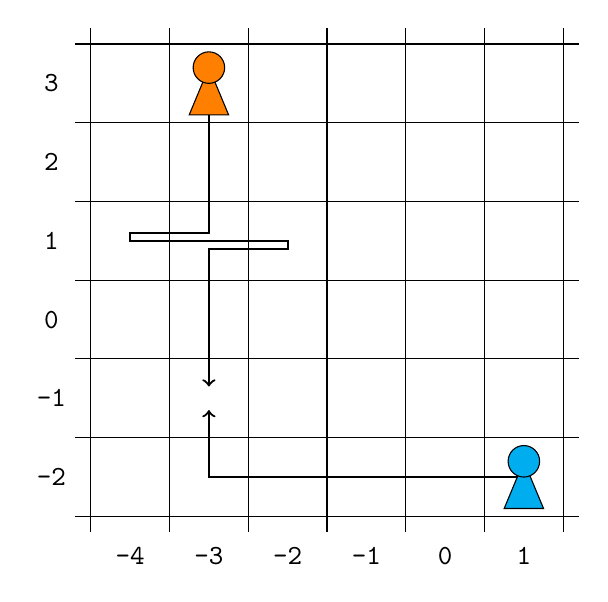
\begin{tikzpicture}
	\newcommand\overhang{0.2};
	\newcommand\xmin{-4};
	\newcommand\xmax{2};
	\newcommand\ymin{-2};
	\newcommand\ymax{4};
	%\fill[gray] (-3,-1) rectangle (-2,0);
	\foreach \i in {\xmin,...,\xmax} {
		\draw (\i, \ymin-\overhang) -- (\i, \ymax+\overhang);
	}
	\foreach \i in {\xmin,...,1} {
		\draw (\i+.5, \ymin-.5) node {\texttt{\i}};
	}
	\foreach \i in {\ymin,...,\ymax} {
		\draw (\xmin-\overhang, \i) -- (\xmax+\overhang, \i);
	}
	\foreach \i in {\ymin,...,3} {
		\draw (\xmin-.5, \i+.5) node {\texttt{\i}};
	}
	\draw[thick,->] (1.5,-1.5) -- (-2.5,-1.5) -- (-2.5,-.65);
	\fill[cyan] (1.25,-1.9) -- (1.75,-1.9) -- (1.5,-1.3) -- cycle;
	\draw (1.25,-1.9) -- (1.75,-1.9) -- (1.5,-1.3) -- cycle;
	\fill[cyan] (1.5,-1.3) circle (.2);
	\draw (1.5,-1.3) circle (.2);
	\draw[thick,->] (-2.5,3.5) -- (-2.5,1.6) -- (-3.5,1.6) -- (-3.5,1.5) -- (-1.5,1.5) -- (-1.5,1.4) -- (-2.5,1.4) -- (-2.5,-.35);
	\fill[orange] (-2.75,3.1) -- (-2.25,3.1) -- (-2.5,3.7) -- cycle;
	\draw (-2.75,3.1) -- (-2.25,3.1) -- (-2.5,3.7) -- cycle;
	\fill[orange] (-2.5,3.7) circle (.2);
	\draw (-2.5,3.7) circle (.2);
\end{tikzpicture}

\end{document}
